\emph{
	Diga por qu\'e el siguiente c\'odigo en Octave simula la trayectoria aproximada del proceso $X$ en el intervalo $[0,1]$.
	\texttt{
		\lstinputlisting{tarea5/problema5_2/SuborEst.m}
	}
}

\afterstatement\pn

Primero se está definiendo el valor de la constante \texttt{C} como \texttt{1}.\pn

\texttt{alpha=1/2;} está definiendo un valor para nuestra variable $\alpha$ (entre 0 y 1, como tendría que ser
para que las variables las variables $X_t$ sean finitas casi seguramente según lo demostrado en [\ref{problema5_2:inciso2}]).\pn

\verb+lambda=C/e^alpha;+
define un valor para $\lambda$.\pn

\texttt{T=1;} se define así porque sólo nos interesa saber que ocurre con nuestro proceso hasta el tiempo $1$.\pn

\texttt{N=poissrnd(lambda*T, 1);} está estimando la cantidad de saltos al tiempo \texttt{T}.\pn

La siguiente parte es la interesante. \verb+dx=e./(rand(N,1).^(1/(alpha)));+ está estimando los incrementos de $X$. 
Se está utilizando el resultado de [\ref{problema5_2:inciso3}]. Donde \verb+rand(N,1).^(1/(alpha))+ no es otra cosa más que $t^{1/\alpha}$. 
Se está suponiendo que los incrementos ``infinitesimales'' de $t^{1/\alpha} X_1$ son tan chiquitos como \texttt{e = 0.000001}. Utilizando esto,
se estiman los incrementos ``infinitesimales'' de $X$.\pn 

El resto del código es únicamente para propósitos de graficación.\pn

A continuación una gráfica que resultó de ejecutar el código.

\begin{center}
    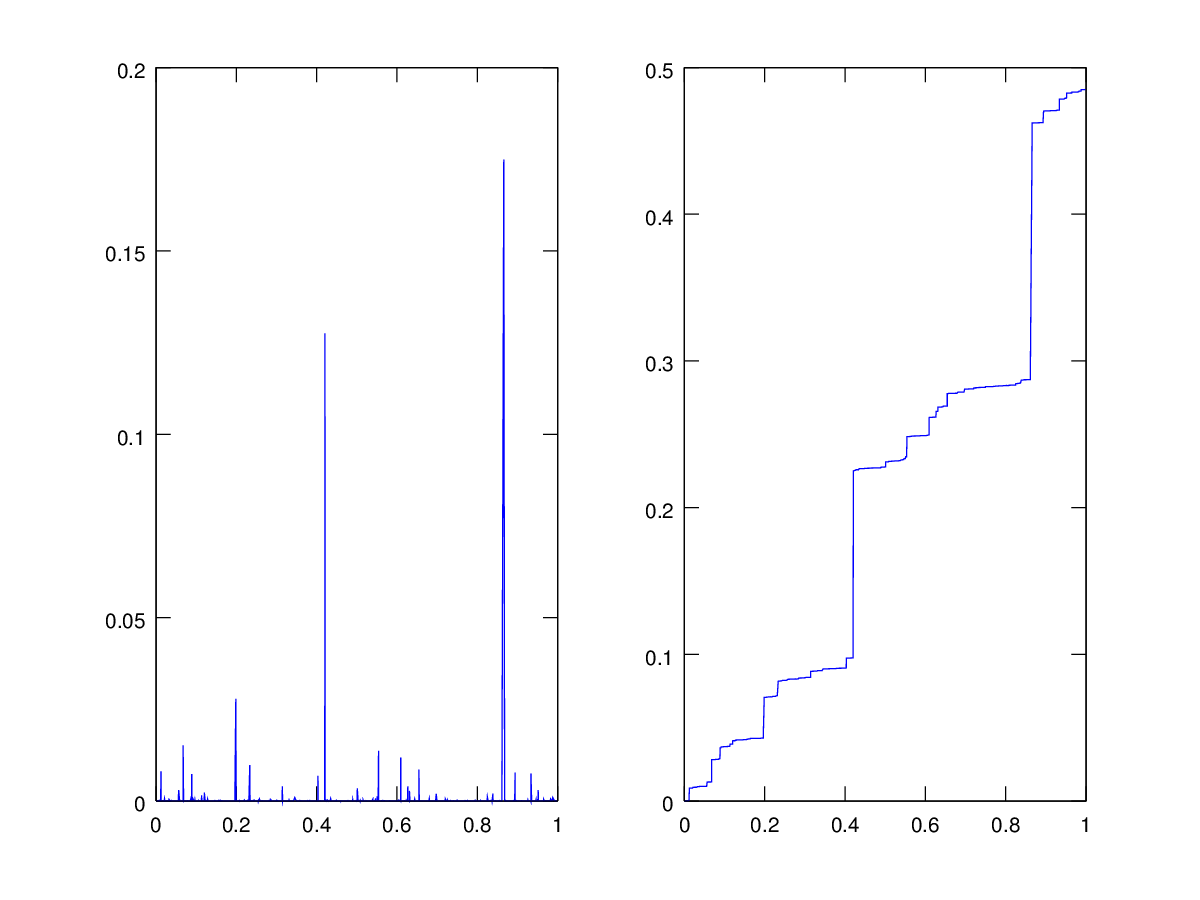
\includegraphics[width=8cm]{tarea5/problema5_2/TrayectoriaAproximadaDeX.png}
\end{center}\pn